% !TEX encoding = UTF-8
% !TEX TS-program = pdflatex
% !TEX root = ../tesi.tex

%**************************************************************
\chapter{Progettazione e codifica}
\label{cap:progettazione e codifica}
%**************************************************************

\intro{In questo capitolo vengono trattati la progettazione e codifica della parte front-end della web-app. Vie }\\

\section{Progettazione}
\subsection{Architettura Angular}
Un'applicazione Angular è formato da un insieme di moduli, dove il modulo pricinpale è il modulo root, chiamato AppModule, che contiene più moduli di funzionalità. Un modulo di funzionalità è composto da un componente, che devinisce la vista dell'utente.
La vista viene modificata da Angular in base alla logica del codice. Ogni componente possiede un template di HTML, dove viene definita il modello di vista, combinata con le direttive di Angular consente di motificare il codice HTML, una volta cambiata la struttura della pagina viene fatto il rendering\gl{} e infine viene cambiata la vista.\\ 
I componenti utilizzano dei servizi che forniscono funzionalità specififche come la login, ma non sono correlate direttamente alla vista, essi sono inseriti come delle dipendenze e grazie a questo rende il codice riutilizzabile ed efficiente. Non solo i servizi sono riutilizzabili ma anche i componenti lo sono, quindi un componente può contenere più componenti così rende l'applicazione Angular più semplice da comprendere e manutenibile in futuro.\\
\begin{figure}[H]
    \centering
    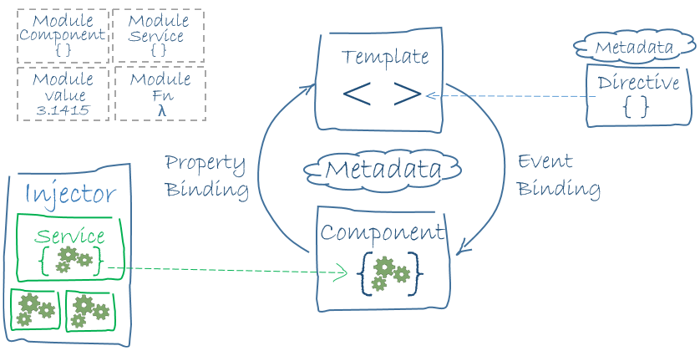
\includegraphics[scale=0.5]{angularArc.png}
    \caption{Architettura Angular}
\end{figure}
\subsection{Architettura SushiLab}
La web-app segue l'architettura spiegata precedentemente che è anche quello consigliato dal sito ufficiale di Angular.\\
Per ogni componente si è creato una cartella per essa, in cui contiene il suoi file .ts per la logica, .html per la struttura, .scss per il layout di grafica e infine i suoi componenti figli. Per i componenti condivisi si è creato una cartella shared dove vengono salvati i componenti che sono utilizzati in più parti dell'applicazione\\
Nella cartella rest vengono salvati tutti i file service, in cui ci sono dei metodi che sono chiamati in più parti dell'applicazione al fine di massimizzare il riuso del codice.\\
\begin{figure}[H]
    \centering
    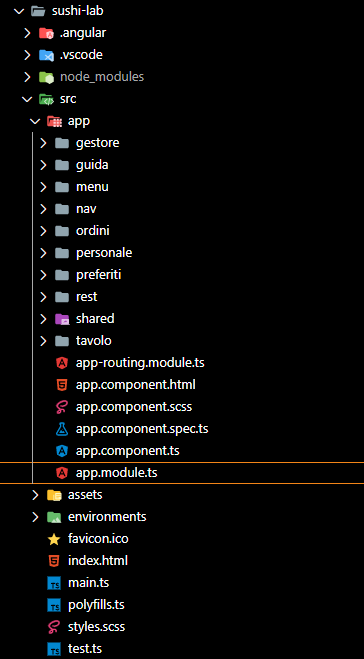
\includegraphics[scale=0.55]{struttura.png}
    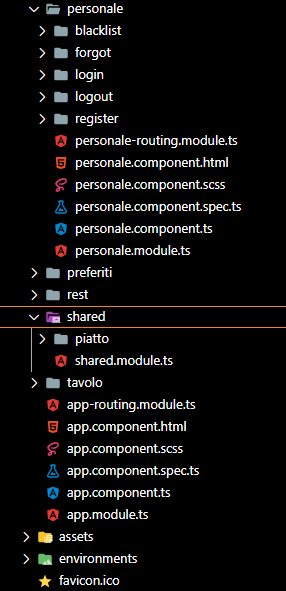
\includegraphics[scale=0.6]{struttura1.png}
    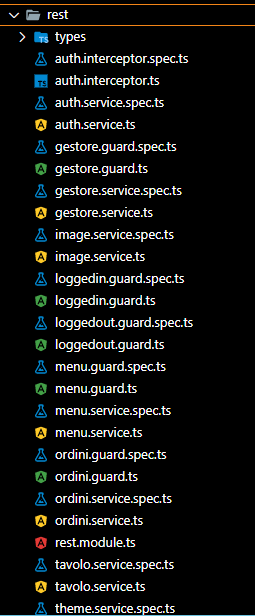
\includegraphics[scale=0.55]{struttura2.png}
    \caption{Struttura file SushiLab}
\end{figure}
\subsection{Progettazione API}
La API sono implementate tramite la piattaforma Stoplight che è uno dei requisiti obbligatori richiesti dall'azienda.\\
La progettazione delle API sono molto semplici grazie all'interfaccia semplice di Stoplight, che permette di definire i path\gl{} e i rispettivi metodi facilmente.\\
Per ogni chiamata bisogna avere:
\begin{itemize}
    \item \textbf{Nome:} individua le API;
    \item \textbf{Descrizione:} spiega in dettaglio la funzione della API;
    \item \textbf{Metodo:} definisce il tipo di chiamata, è stato usato:
    \begin{itemize}
        \item  \textbf{get:} per richiedere dei dati al server come la chiamata per ottenere il menù;
        \item  \textbf{post:} per inviare dei dati sintetici al server come i dati per login;
        \item  \textbf{delete:} per eliminare dei dati dal server come eliminazione della sessione di tavolo;        
    \end{itemize};
    \item \textbf{Path:} definisce il percorso finale della API;
    \item \textbf{Risposta:} configura la risposta che ritorna la API, è stato usato:
    \begin{itemize}
        \item  \textbf{200:} richiesta andata a buon fine;
        \item  \textbf{201:} creazione andata a buon fine;
        \item  \textbf{204:} richiesta andata a buon fine ma il contenuto è vuoto;
        \item  \textbf{401:} non autorizzato;
        \item  \textbf{404:} non trovato;
        \item  \textbf{406:} non accettato;
        \item  \textbf{500:} errore interno;
    \end{itemize}
\end{itemize}
\begin{figure}[H]
    \centering
    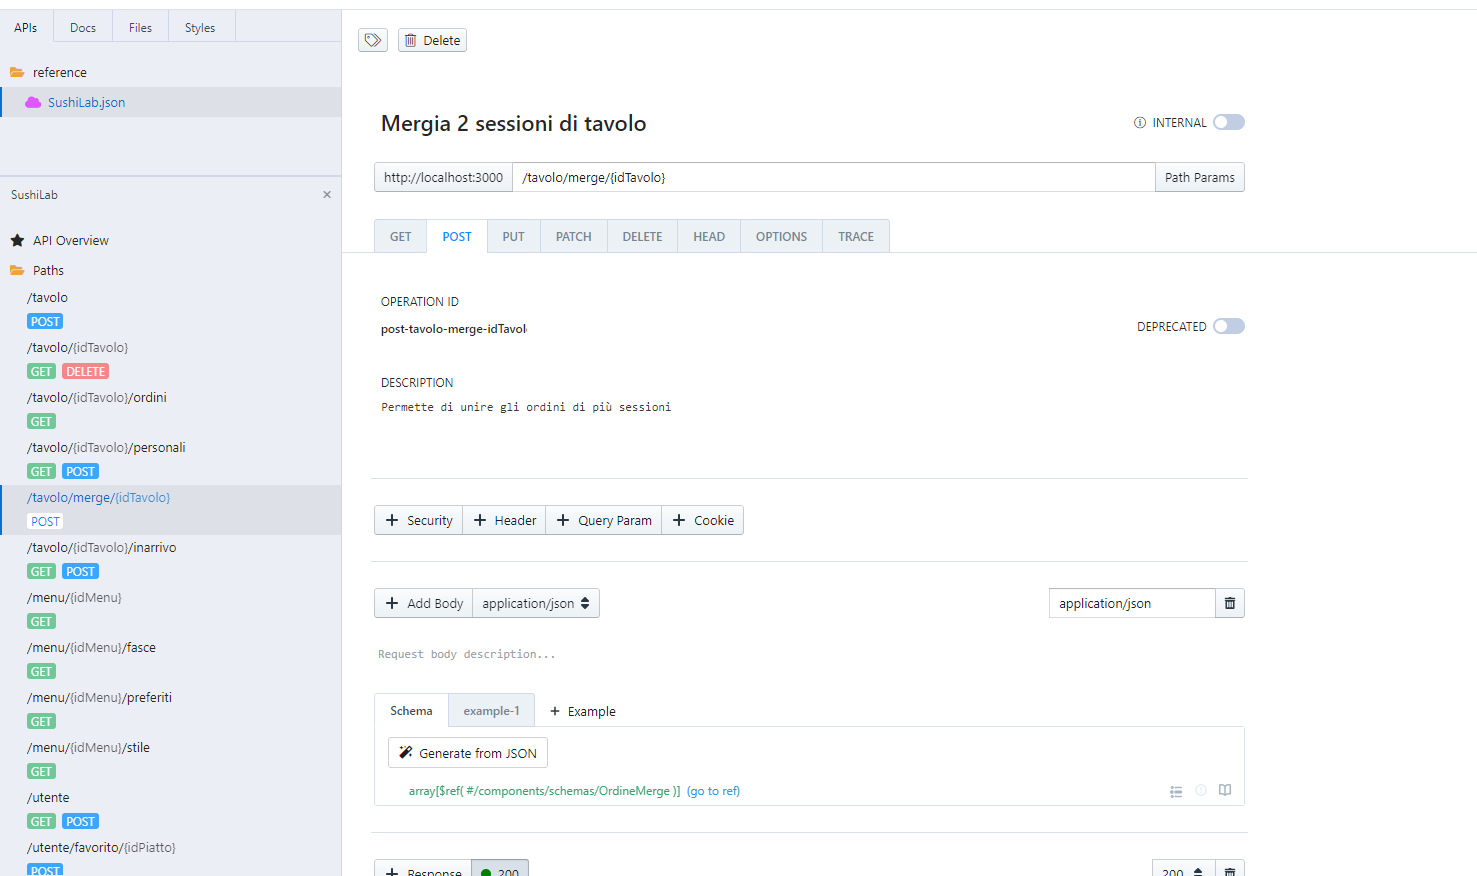
\includegraphics[scale=0.55]{stoplight.png}
    \caption{Stoplight SushiLab}
\end{figure}
\subsection{Progettazione delle viste}
All'inizio si è fatto un meeting\gl{} con il tutur aziendale per chiarire le funzionalità che deve avere la web-app, dopo di che si è iniziato la progettazione delle viste tramite la editor di grafica online\gl{} Figma\gl{}.\\
Tramite il sistema di progettazione di Figma sono stati creati le bozze delle viste per chiarire i collegamenti tra di loro e i posizionamenti dei compoenti. 
Il posizionamento dei componenti sono scelti in base al loro numero di volte che viene premuto e si è anche basato alle web-app più popolari.
È stato deciso i seguenti aspetti:
\begin{itemize}
    \item I colori principali e lo sfondo della applicazione;
    \item Il bottone per la navbar\gl{} è in alto a destra;
    \item Il logo della piattaforma in alto a sinistra;
    \item I bottoni, testi e form devono avere lo stesso stile e colore in base alla loro funzionalità;
    \item Lo stile del piatto in modalità dettaglio in menù e nella lista degli ordini personali è la stessa;
    \item Tutti le maschere hanno una visuale che utilizza la card.
\end{itemize}
\begin{figure}[H]
    \centering
    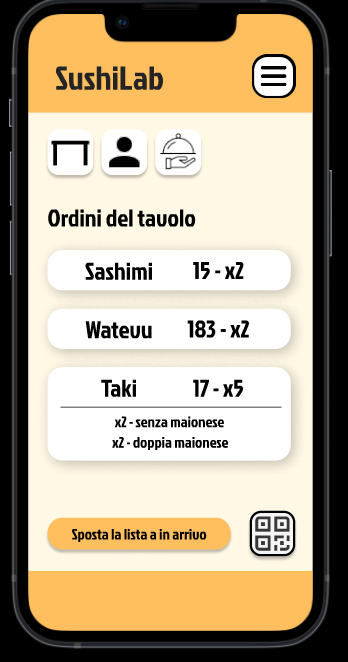
\includegraphics[scale=1]{figma.png}
    \caption{Figma SushiLab}
\end{figure}


% {\hyperref[cap:menu.component]{Il secondo capitolo}}
\section{Codifica}
\subsection{Interfaccie}
\subsubsection{Menù}
Viene mostrata il menù del ristorante che comprende tutte le categorie e le loro piatti.\\
\textbf{Funzionalità:}
\begin{itemize}
    \item L'utente può aumentare la quantità di un piatto per aggiungerlo o aumentare la sua quantità nell'ordine del tavolo;
    \item L'utente può diminuire la quantità di un piatto per rimuoverlo o diminuire la sua quantità nell'ordine del tavolo;
    \item L'utente può visualizzare il piatto in modalità dettaglio per dare una recensione al piatto o inserisce una nota per il piatto;
    \item L'utente può aggiungere il piatto nella lista dei preferiti o rimuoverlo dalla lista.
\end{itemize}
\begin{figure}[H]
    \centering
    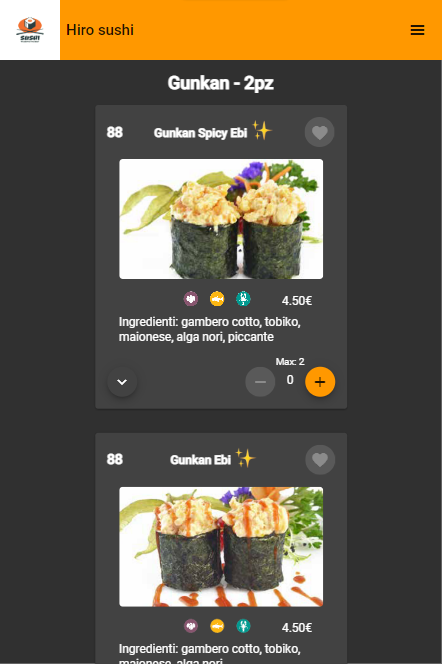
\includegraphics[scale=.6]{menu.png}
    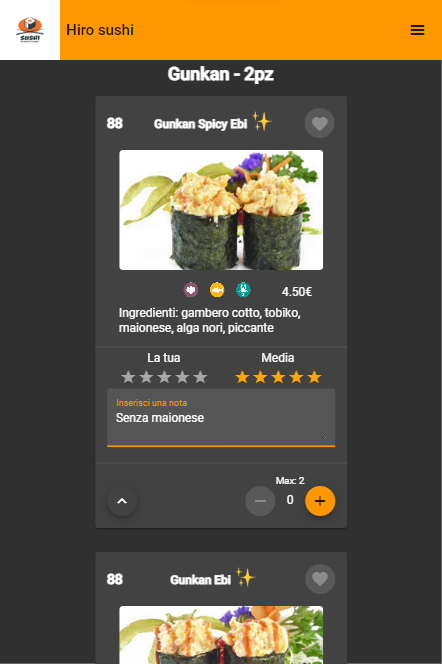
\includegraphics[scale=.6]{menu2.png}
    \caption{Menù e Menù con piatto in dettaglio di SushiLab}
\end{figure}
\subsubsection{Gestione tavolo}
Viene mostrata la maschera di gestione tavolo.\\
\textbf{Funzionalità:}
\begin{itemize}
    \item L'utente può creare una sessione di tavolo;
    \item L'utente può andare al form per unire ad una sessione.
\end{itemize}
\begin{figure}[H]
    \centering
    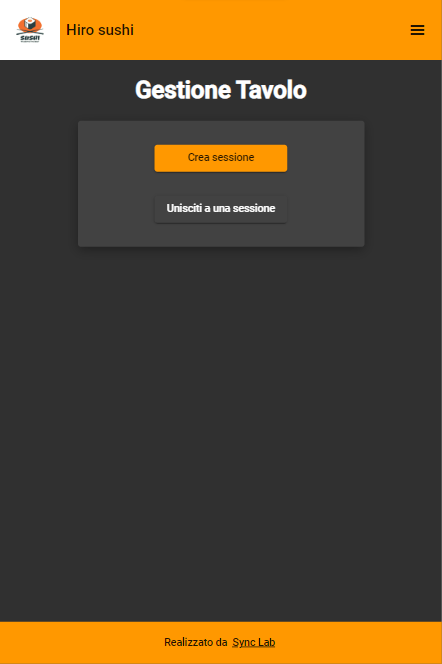
\includegraphics[scale=.6]{gestione tavolo.png}
    \caption{Menù SushiLab}
\end{figure}
\subsubsection{Unisci sessione}
Interfaccia tramite la quale è possibile unire ad una sessione di tavolo.\\
\textbf{Funzionalità:}
\begin{itemize}
    \item L'utente può  unirsi ad una sessione inserendo il codice di sessione se il codice non rispetta la validazione del form non si abilita il bottone unisci;
    \item L'utente può tornare nella pagina gestione tavolo.
\end{itemize}
\begin{figure}[H]
    \centering
    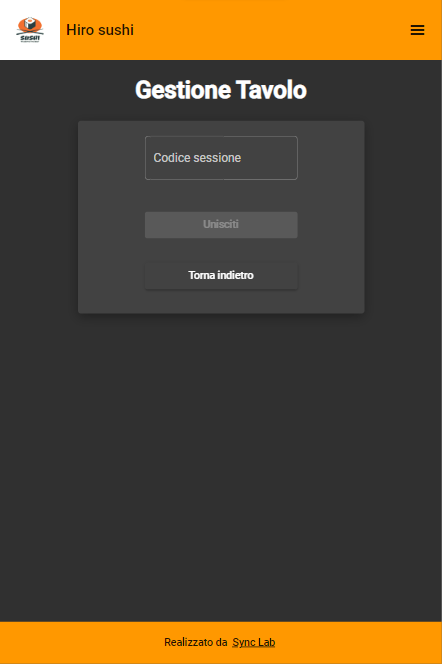
\includegraphics[scale=.6]{unisci.png}
    \caption{Menù SushiLab}
\end{figure}
\subsubsection{QR-code tavolo}
Viene mostrata il QR-code del tavolo che permette agli altri utenti che si trovano sullo stesso tavolo dell'untente di unirsi.\\
\textbf{Funzionalità:}
\begin{itemize}
    \item L'utente può uscire dalla sessione premendo il bottone esci dalla sessione.
\end{itemize}
\begin{figure}[H]
    \centering
    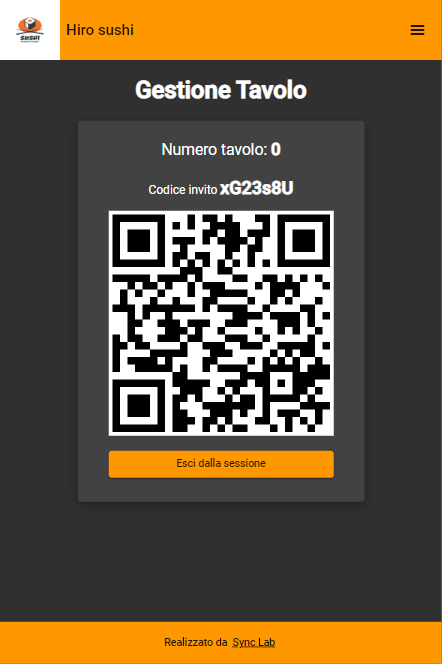
\includegraphics[scale=.6]{gestionetavolo2.png}
    \caption{Menù SushiLab}
\end{figure}
\subsubsection{Lista ordini del tavolo}
Viene mostrato la lista degli ordini della sessione del tavolo in cui si trova l'utente.\\
\textbf{Funzionalità:}
\begin{itemize}
    \item L'utente può spostare la lista in arrivo;
    \item L'utente può generare il QR-code premendo sul bottone QR-code;
    \item L'utente può andare in altri sezioni della lista ordini utilizzando la navbar interna.
\end{itemize}
\begin{figure}[H]
    \centering
    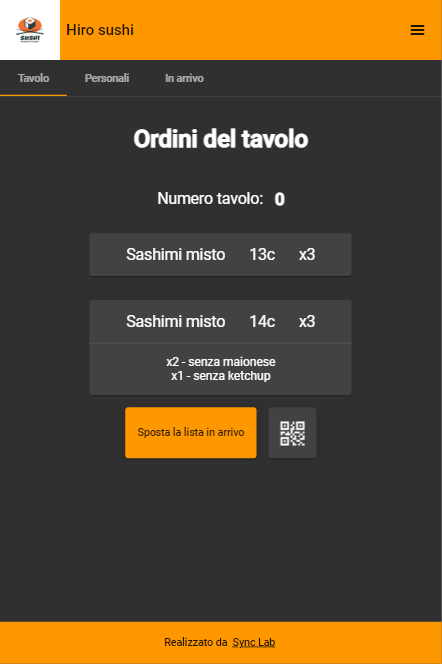
\includegraphics[scale=.6]{ordinitavolo.png}
    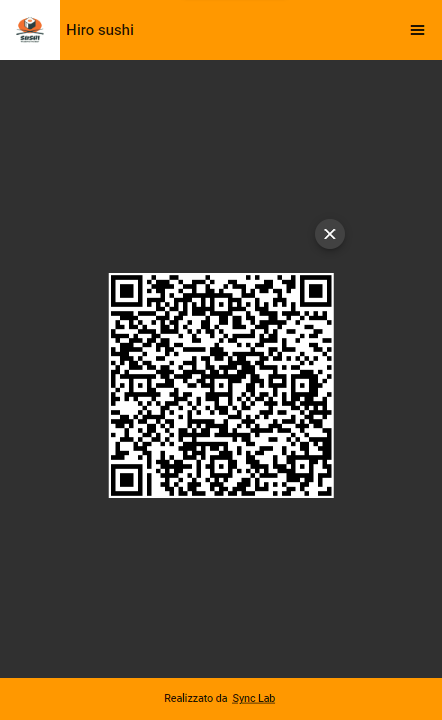
\includegraphics[scale=.6]{ordinitavolo2.png}
    \caption{Menù SushiLab}
\end{figure}
\subsubsection{Lista ordini personali}
Viene mostrata la lista degli ordini personali.\\
\textbf{Funzionalità:}
\begin{itemize}
    \item L'utente può visualizzare i piatti in modalità dettaglio;
    \item L'utente può visualizzare i piatti in modalità normale;
    \item L'utente può aggiungere un piatto nella lista dei preferiti o rimuoverlo dalla lista;
    \item L'utente può dare una recensione ad un piatto.
\end{itemize}
\begin{figure}[H]
    \centering
    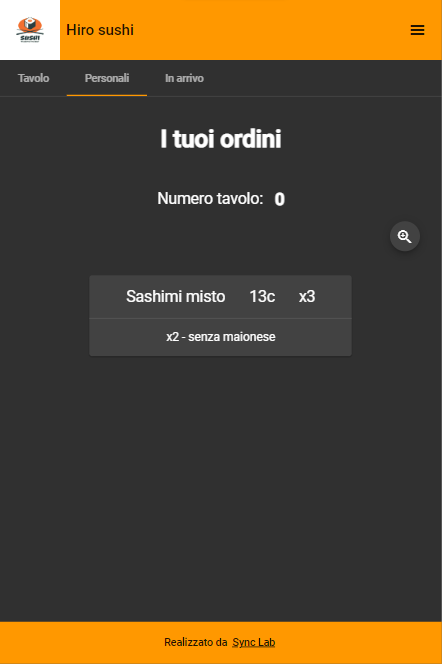
\includegraphics[scale=.6]{ordinipersonali.png}
    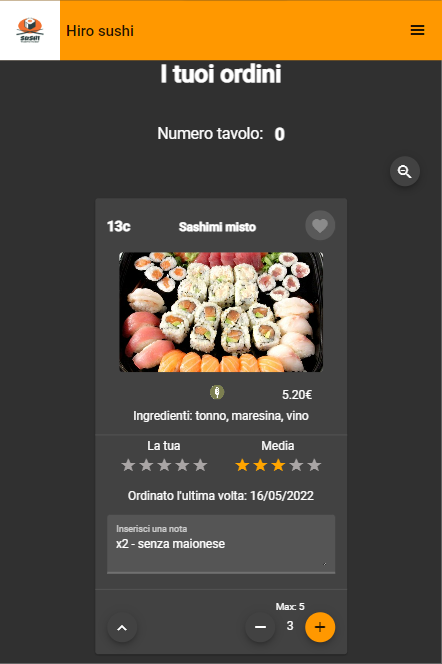
\includegraphics[scale=.6]{ordinipersonali2.png}
    \caption{Menù SushiLab}
\end{figure}
\subsubsection{Lista ordini in arrivo}
Viene mostrata la lista degli ordini in arrivo.\\
\textbf{Funzionalità:}
\begin{itemize}
    \item L'utente può visualizzare i piatti in modalità dettaglio;
    \item L'utente può visualizzare i piatti in modalità normale;
    \item L'utente può marcare un piatto come arrivato;
    \item L'utente può aggiungere un piatto nella lista dei preferiti o rimuoverlo dalla lista;
    \item L'utente può dare una recensione ad un piatto.
\end{itemize}
\begin{figure}[H]
    \centering
    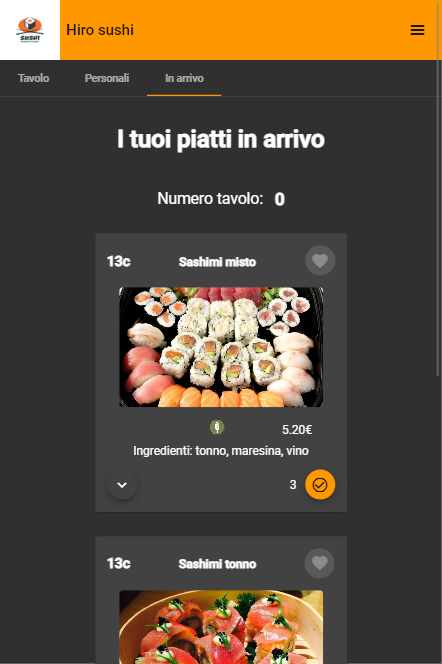
\includegraphics[scale=.6]{ordiniinarrivo.png}
    \caption{Menù SushiLab}
\end{figure}
\subsubsection{Login}
Viene mostrato il form per effetture il login dove è possibile effettuare la login nella piattaforma.\\
\textbf{Funzionalità:}
\begin{itemize}
    \item L'utente può effettuare il login inserendo i campi correttamente altrimenti viene evidenziato in rosso i campi sbagliati;
    \item L'utente può andare al form di registrazione;
    \item L'utente può andare al form di password dimenticata.
\end{itemize}
\begin{figure}[H]
    \centering
    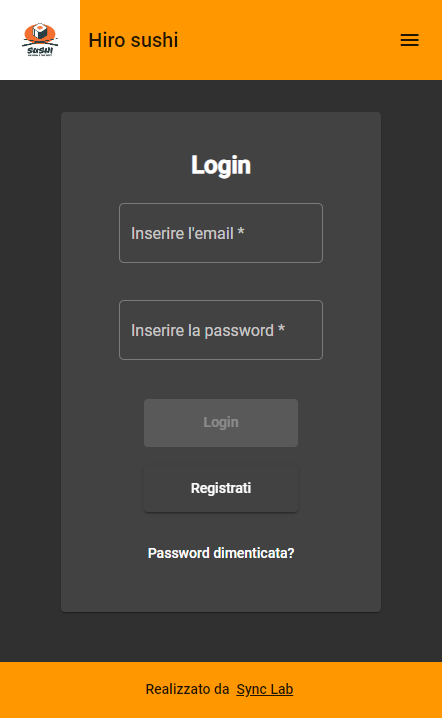
\includegraphics[scale=.6]{login.png}
    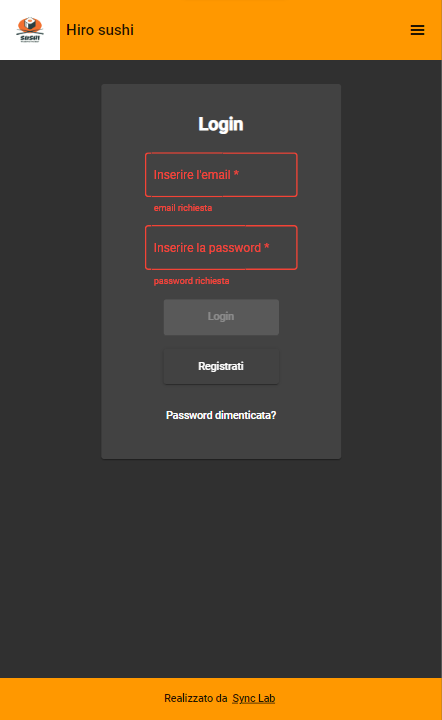
\includegraphics[scale=.6]{login2.png}
    \caption{Menù SushiLab}
\end{figure}
\subsubsection{Registrazione}
Viene mostrato il form di registrazione dove è possibile registrare nella piattaforma.\\
\textbf{Funzionalità:}
\begin{itemize}
    \item L'utente può effettuare la registrazione inserendo i campi correttamente altrimenti viene evidenziato in rosso i campi sbagliati;
    \item L'utente può andare al form di login.
\end{itemize}
\begin{figure}[H]
    \centering
    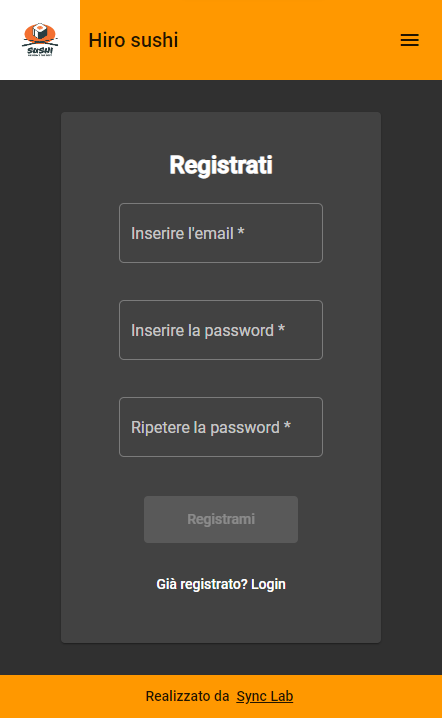
\includegraphics[scale=.6]{registrati.png}
    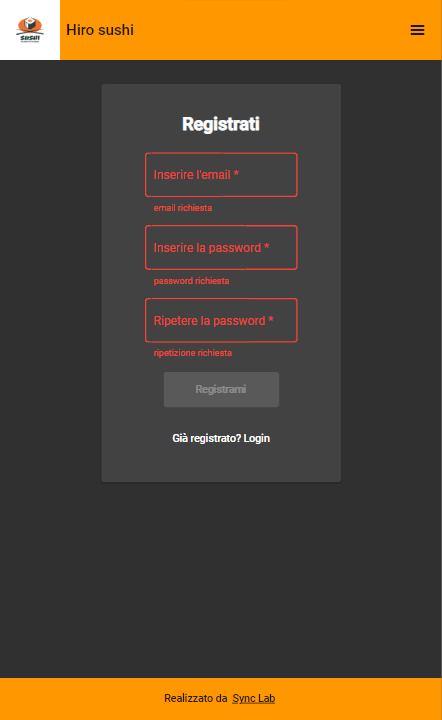
\includegraphics[scale=.6]{registrati2.png}
    \caption{Menù SushiLab}
\end{figure}
\subsubsection{Password Dimenticata}
Viene mostrato il form di cambia password dove è possibile reimpostare la password.\\
\textbf{Funzionalità:}
\begin{itemize}
    \item L'utente può reimpostare la password inserendo i campi correttamente altrimenti viene evidenziato in rosso i campi sbagliati;
    \item L'utente può andare al form di registrazione;
    \item L'utente può andare al form di Login.
\end{itemize}
\begin{figure}[H]
    \centering
    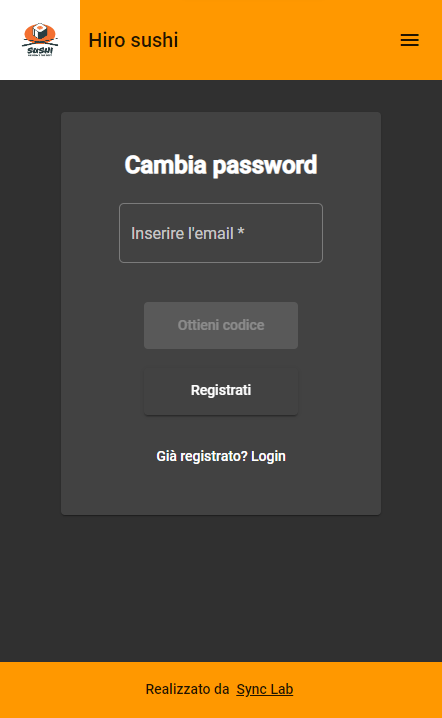
\includegraphics[scale=.6]{cambiapass.png}
    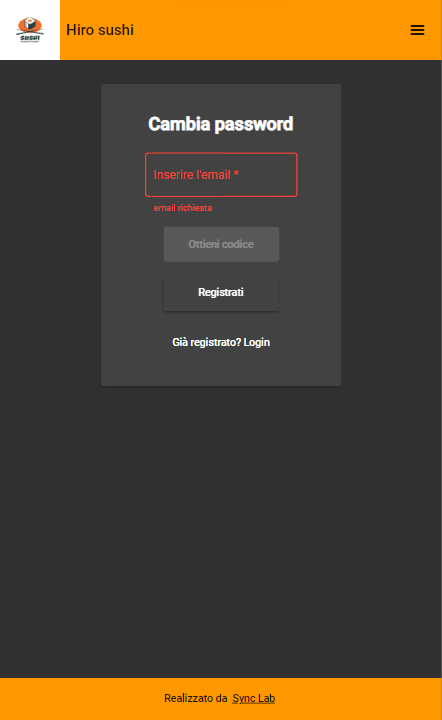
\includegraphics[scale=.6]{cambiapass2.png}
    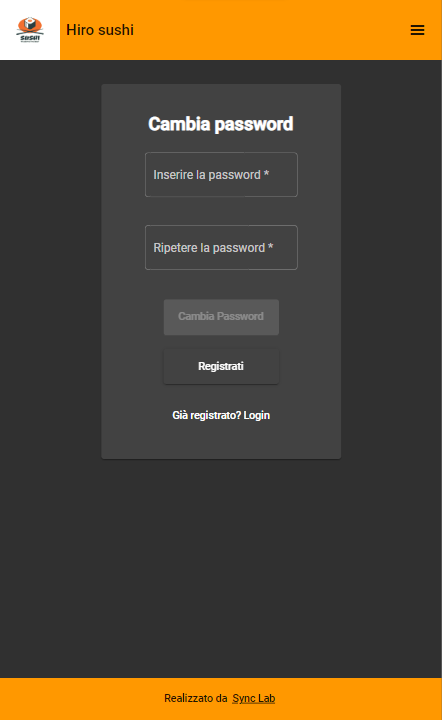
\includegraphics[scale=.6]{cambiapass3.png}
    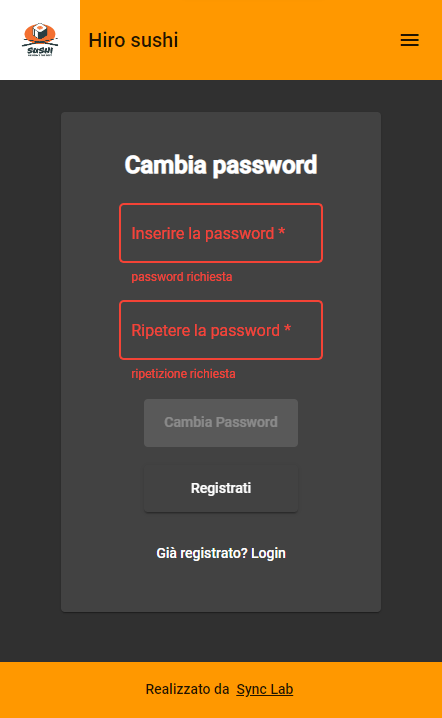
\includegraphics[scale=.6]{cambiapass4.png}
    \caption{Menù SushiLab}
\end{figure}
\subsubsection{Area Personale}
Viene mostrata l'area personale dell'utente dove si può vedere i dati dell'utente.
\textbf{Funzionalità:}
\begin{itemize}
    \item L'utente può effettuare il logout;
    \item L'utente può andare nella sezione di blacklist ingredienti per inserire o rimuovere delle allergeni o preferenze.
\end{itemize}
\begin{figure}[H]
    \centering
    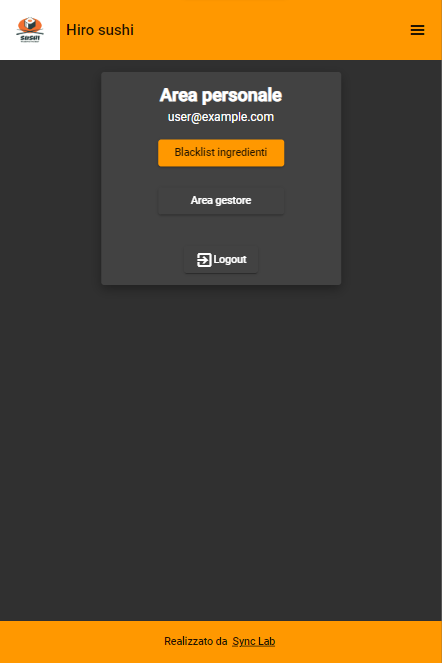
\includegraphics[scale=.6]{personale.png}
    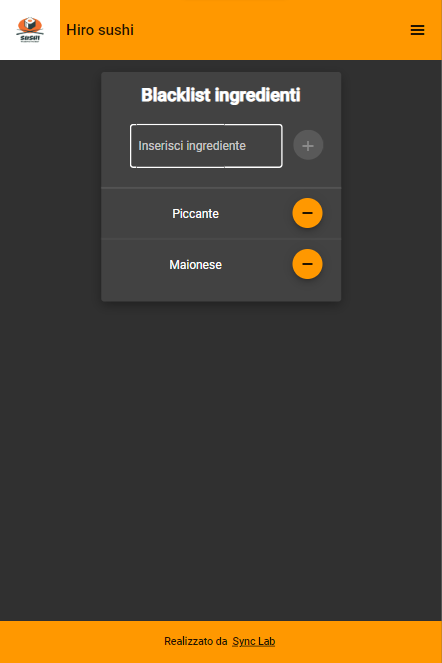
\includegraphics[scale=.6]{blacklist.png}
    \caption{Menù SushiLab}
\end{figure}
\label{cap:menu.component}